Nessa tarefa o nosso interesse é estudar o fenômeno de quebra espontânea de simetria. 
Queremos mostrar que o tempo que um sistema leva para mudar toda a orientação de magnetização cresce de forma 
exponencial com a dimensão da malha utilizada. 
Para isso foi implementado uma simulação que executa passos de Monte Carlo e contabiliza o intervalo 
de tempo de Monte Carlo que o sistema leva para mudar a magnetização conforme o tamanho $L$ da rede aumenta. 

O código em fortran para essa simulação está abaixo: 

\begin{minted}{fortran}
    implicit integer(f-f)
    implicit real(m-m)
    parameter(L = 100)
    dimension exps(-4:4)
    byte lattice(1:L, 1:L)
    ! periodic boundary conditions
    dimension ipbc(0:L+1)
    ! this or using mod
    open(unit=1, file="saidas/tarefa-4/saida-tarefa-D.dat")
    open(unit=2, file="saidas/tarefa-4/saida-tarefa-MAG_T.dat")
    beta = 0.5
    call define_exponentials(exps, beta)
    do L_real = 4, 10
        print *, "L = ", L_real 
        call srand(3519) ! /L_real+1)
        N = L_real * L_real
        ! setting ipbc
        do i = 1, L_real
            ipbc(i) = i
        end do  
        ipbc(0) = L_real
        ipbc(L_real+1) = 1
        mag = 0.0e0
        call initialize_random_lattice(lattice, L_real, L_real)
        call total_magnetization(lattice, mag, L_real)
        n_inversions = 10000
        n_curr = 0
        n_time = 0
        do while(n_curr < n_inversions) 
            mag_prev = mag
            do i = 1, N
                call flip_spin(lattice, ipbc, exps, E, mag, L_real)
            end do
            n_time = n_time + 1
            ! Fazer o gráfico da magnetização aqui.
            if(mag_prev * mag < 0) then 
                t_mean = t_mean + n_time
                n_time = 0
                n_curr = n_curr + 1
            end if
        end do
        write(2, *) t_mean, mag
        t_mean = t_mean / n_inversions
        write(1, *) L_real, t_mean
    end do
    close(1)
    end
\end{minted}

Podemos ver pela figura(\ref{fig:d_graficos}) que o intervalo cresce de forma exponencial com 
o tamanho $L$ da malha: 

\begin{figure}
    \centering
    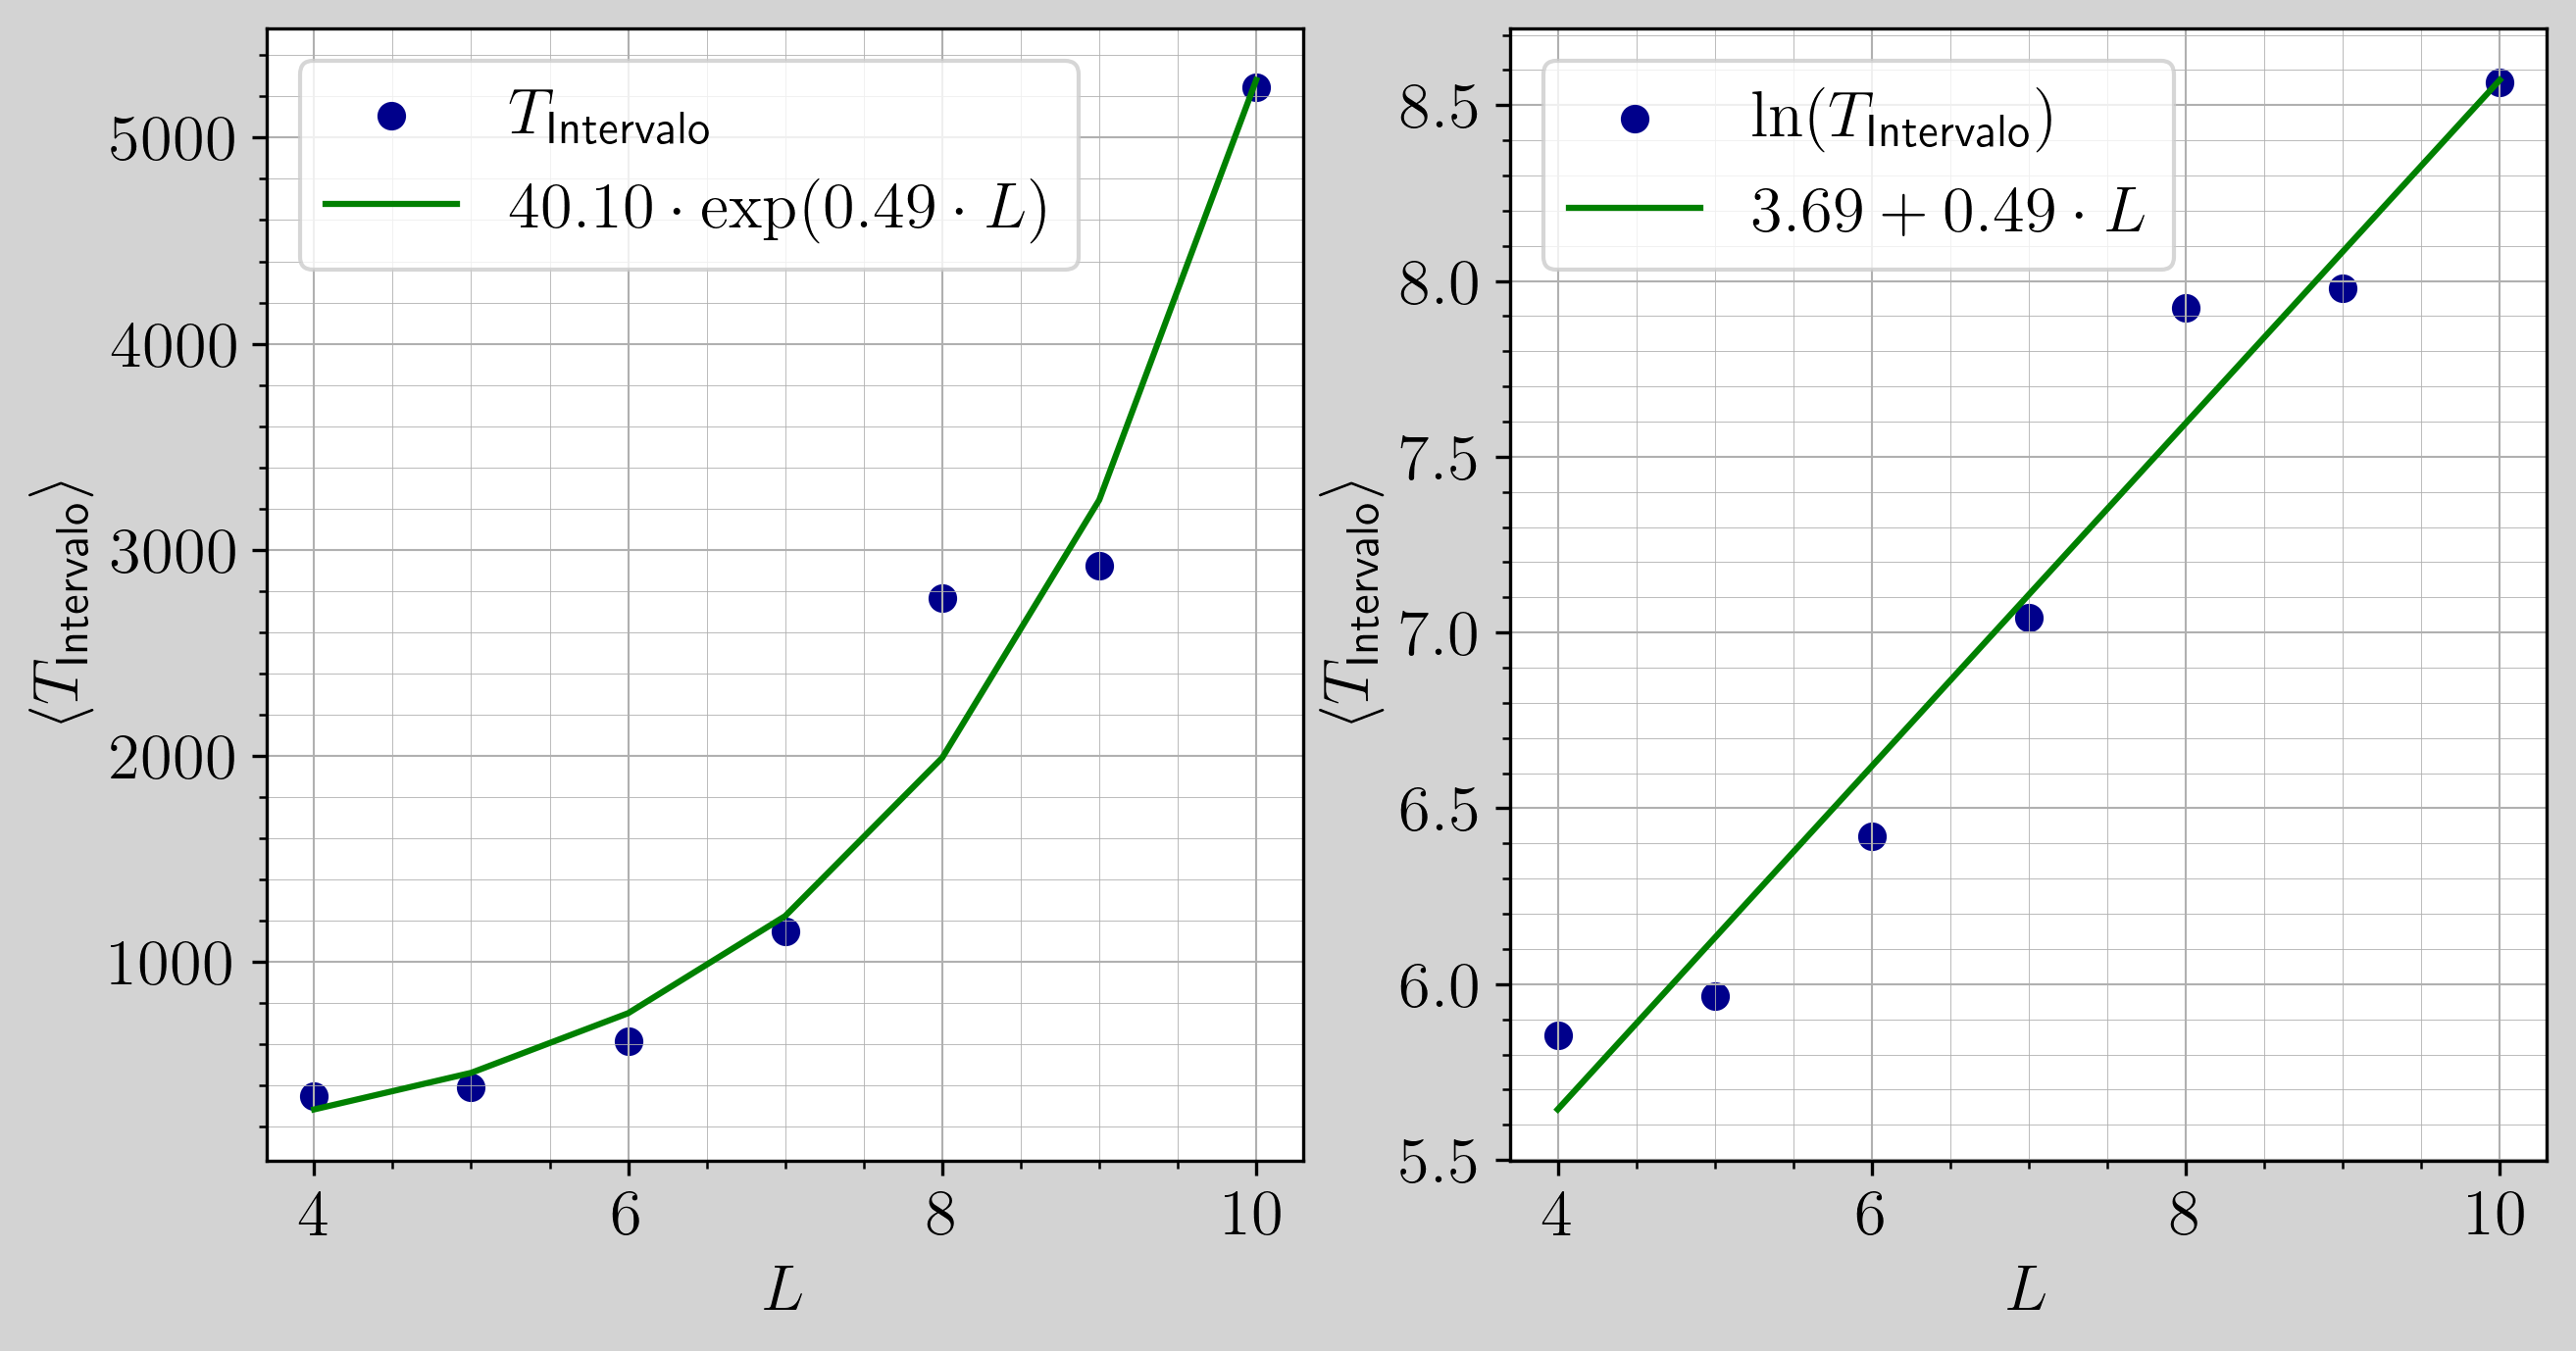
\includegraphics[width=\linewidth]{graficos/tarefa-4/graf-tarefa-D.png}
    \caption{Gráfico do crescimento do intervalo $\langle T_\text{intervalo} \rangle$ em função de $L$ e ajuste linear.}
    \label{fig:d_graficos}
\end{figure}

Para implementação com número de inversões da ordem de $10^4$ foi obtido o ajuste linear 
$\ln\left(\langle T_{\text{intervalo}}(L)\rangle\right)  \approx 3,67 + 0,49 \cdot L$. 

Essa dependência exponencial para que ocorra quebra da simetria talvez explique o que ocorre na simulação da tarefa B
em que o sistema atinge o equilibrio mas a magnetização tem comportamento não usual. Aumentando o número de passos 
de Monte Carlo naquela simulação pode resolver o aparente problema.